\section{Results of basic part}
\subsection{Correctness}
All indexes  of the basic part passed all levels of the correctness test.

\subsection{Time complexity}
\subsubsection{Indexing time}
Figure \ref{fig:BPindextime2}, \ref{fig:BPindextime3}, \ref{fig:BPindextime45} shows the indexing time for index 2,3,4 and 5. Notice that the y-axis varies from plot to plot. Figure \ref{fig:BPindextime2345} shows all indexes compared to each other on a log-transformed plot to compare them against each other.


\begin{figure}[H]
    \centering
     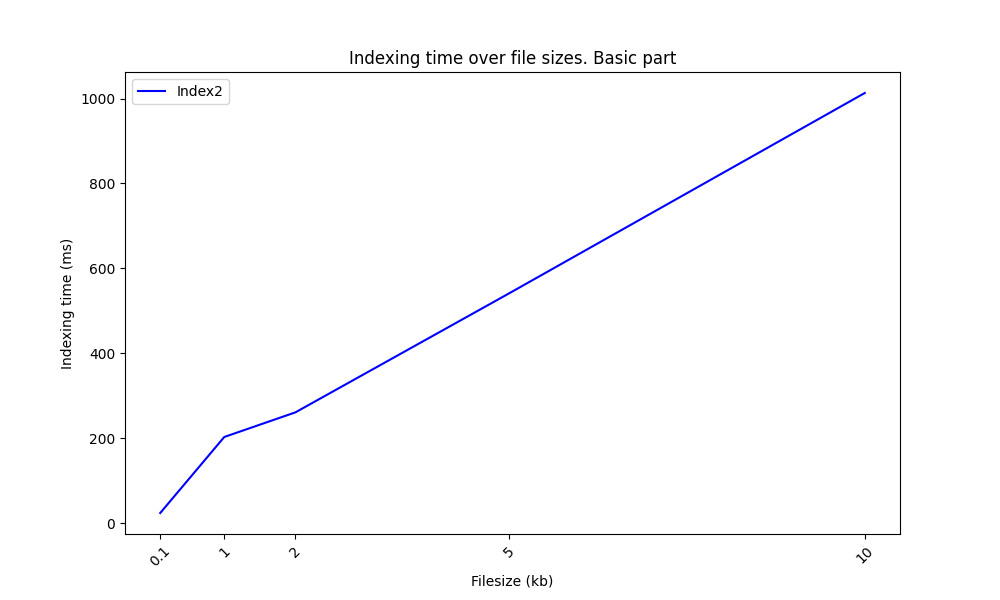
\includegraphics[width=0.8\textwidth]{LaTeX/Figures/BasicPart/BPIndexing[2].png}
    \caption{Indexing time for index 2 over different filesizes}
    \label{fig:BPindextime2}
\end{figure}

\begin{figure}[H]
    \centering
    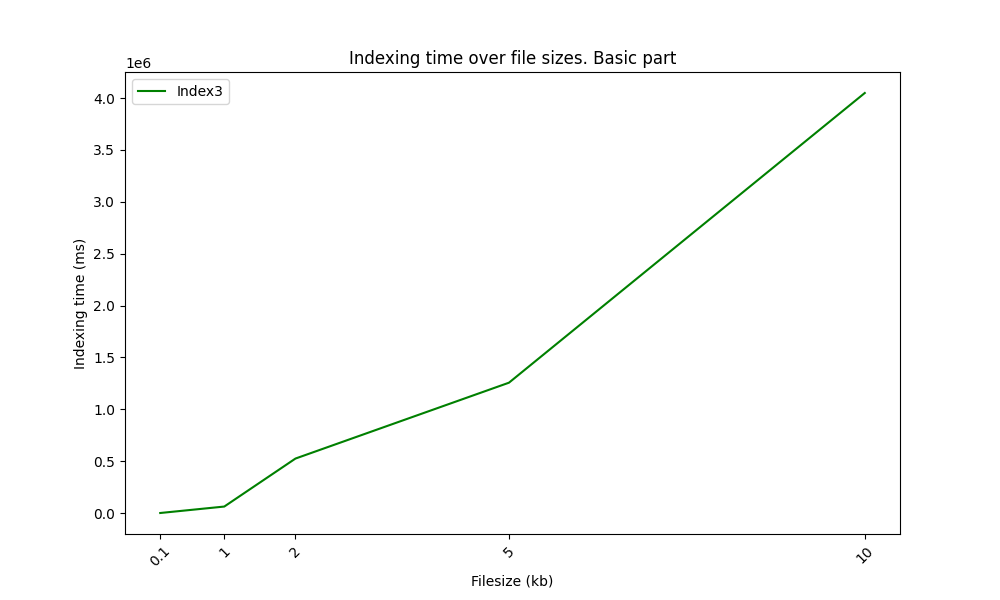
\includegraphics[width=0.8\textwidth]{LaTeX/Figures/BasicPart/BPIndexing[3].png}
    \caption{Indexing time for index 2 over different filesizes}
    \label{fig:BPindextime3}
\end{figure}

\begin{figure}[H]
    \centering
    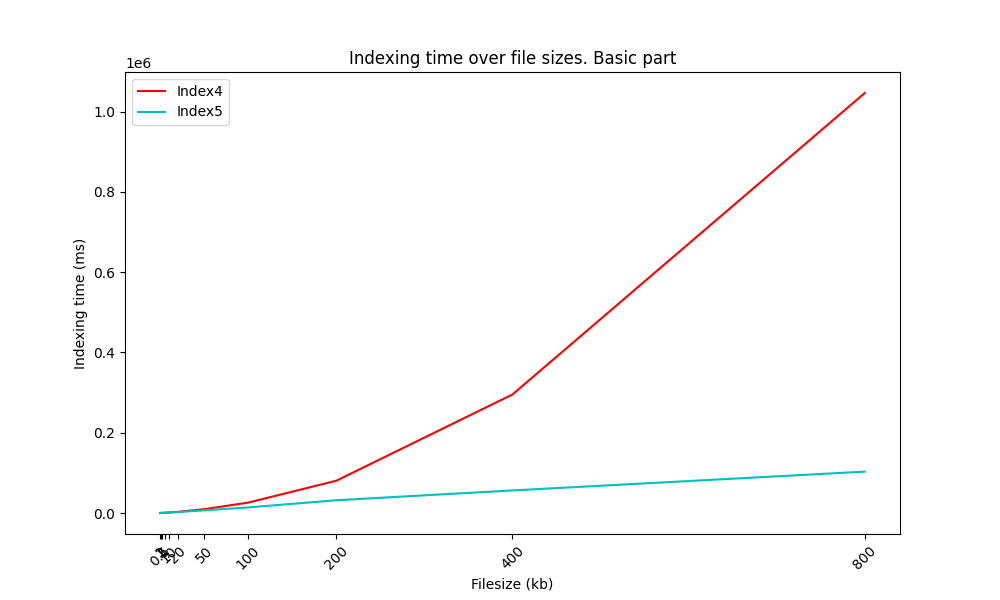
\includegraphics[width=.8\textwidth]{LaTeX/Figures/BasicPart/BPIndexing[4, 5].png}
    \caption{Indexing time for index 2 over different filesizes}
    \label{fig:BPindextime45}
\end{figure}

\begin{figure}[H]
    \centering
    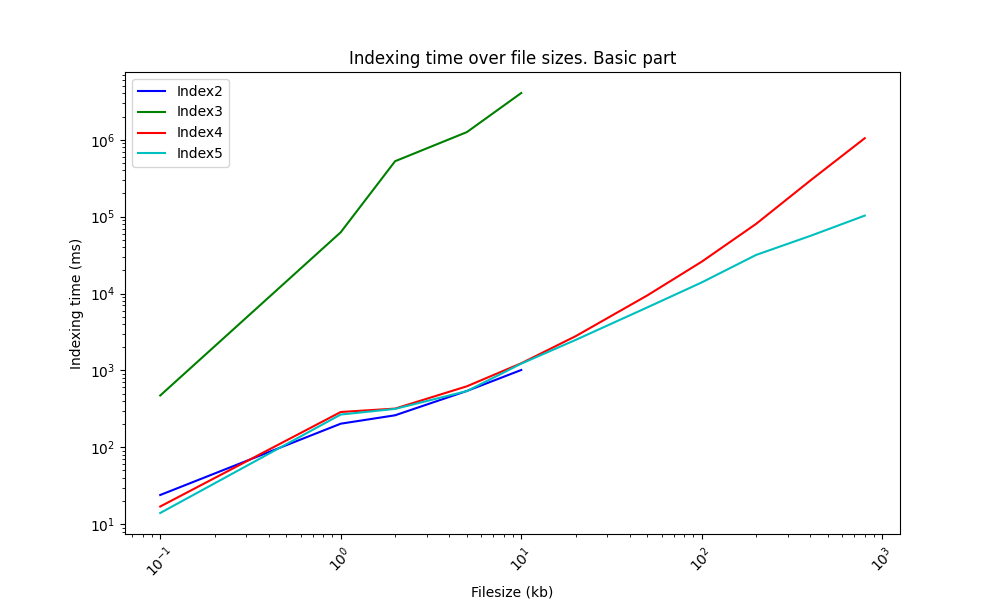
\includegraphics[width=.8\textwidth]{LaTeX/Figures/BasicPart/BPIndexing[2, 3, 4, 5].png}
    \caption{Indexing time for index 2 over different filesizes}
    \label{fig:BPindextime2345}
\end{figure}

\subsubsection{Search time}
Figure \ref{fig:BPindextime2} ans \ref{fig:BPindextime3}, shows the searching time for index 2,3,4 and 5.

\begin{figure}[H]
    \centering
    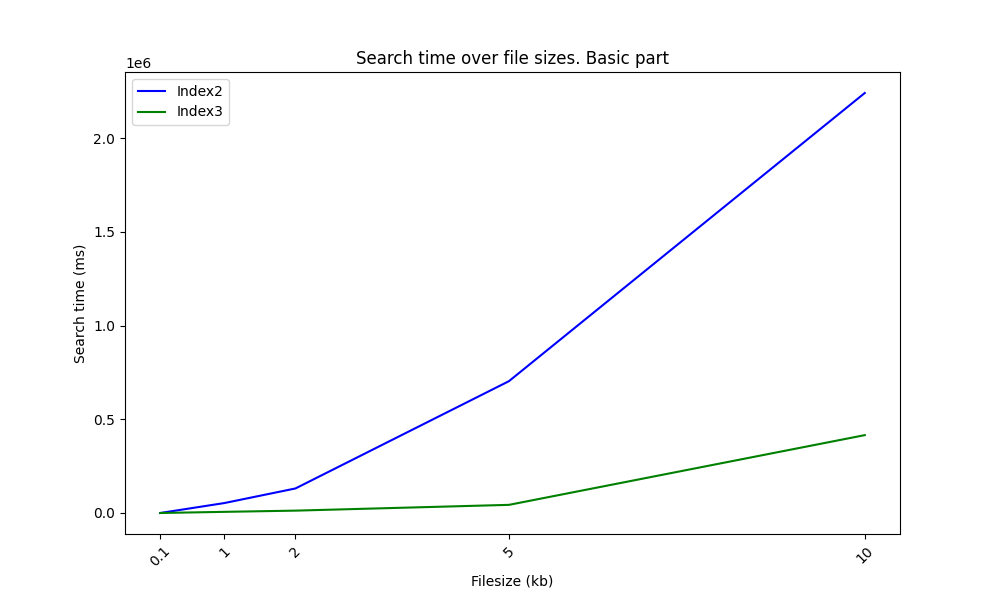
\includegraphics[width=.8\textwidth]{LaTeX/Figures/BasicPart/BPSearch[2, 3].png}
    \caption{Searching time for searching for all unique words in each file for index2 and index3 over different filesizes}
    \label{fig:BPsearch23}
\end{figure}

\begin{figure}[H]
    \centering
    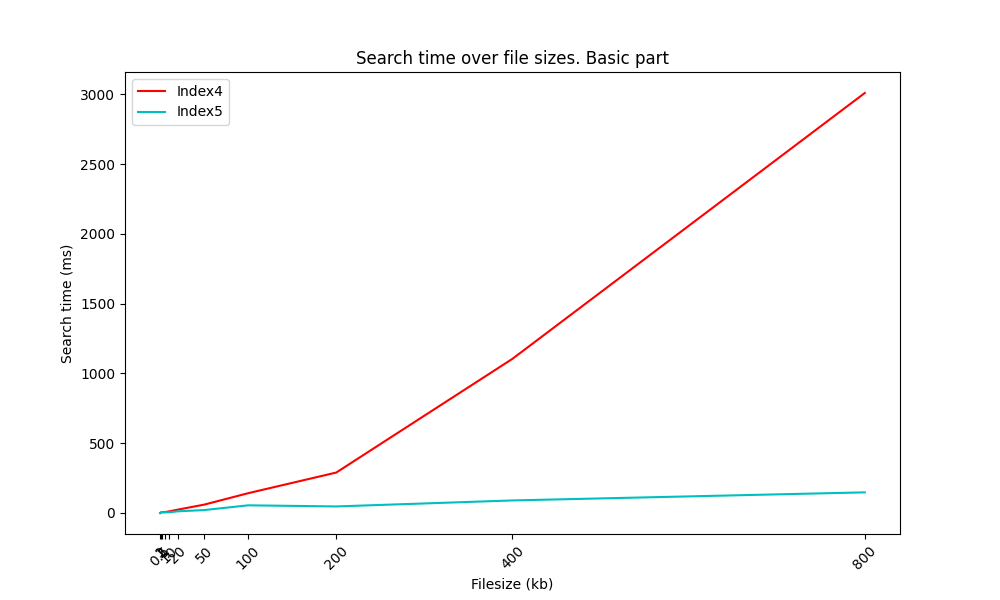
\includegraphics[width=.8\textwidth]{LaTeX/Figures/BasicPart/BPSearch[4, 5].png}
    \caption{Searching time for searching for all unique words in each file for index4 and index5 over different filesizes}
    \label{fig:BPsearch45}
\end{figure} 




